\section{Performance Evaluation}

%% CACHE_MISS
\begin{table}
    \centering
    \fontsize{11}{11}
    \begin{tabular}{| l | r | r | r | r | } %% KVS cache-ref cache-miss 
    \hline
    \footnotesize{\textbf{Workload}} & \footnotesize{\textbf{OPs}} & \footnotesize{\textbf{Footprint(Data)}} & \footnotesize{\textbf{Footprint(Index)}} \\ \hline \hline
    \footnotesize{sequential} & \footnotesize{2M} & \footnotesize{0,000} & \footnotesize{00,000} \\ \hline
    \footnotesize{random} & \footnotesize{2M} & \footnotesize{0,000} & \footnotesize{00,000} \\ \hline
    \footnotesize{webserver} & \footnotesize{2M} & \footnotesize{5.2G} & \footnotesize{5.8G} \\ \hline
    \footnotesize{fileserver} & \footnotesize{2M} & \footnotesize{1.9G} & \footnotesize{2.2G} \\ \hline
    \footnotesize{linkbench run} & \footnotesize{2M} & \footnotesize{5.0G} & \footnotesize{14.8G} \\ \hline
    \footnotesize{tpcc} & \footnotesize{2M} & \footnotesize{2.7G} & \footnotesize{5.8G} \\ \hline
%    \footnotesize{sequential} & \footnotesize{29,831} & \footnotesize{4,125} & \footnotesize{21,986} & \footnotesize{2,731} \\ \hline 
%    \footnotesize{random} & \footnotesize{38,272} & \footnotesize{5,810} & \footnotesize{20,949} & \footnotesize{2,727} \\ \hline 
%    \footnotesize{linkbench} & \footnotesize{9,238} & \footnotesize{4,368} & \footnotesize{4,844} & \footnotesize{1,938} \\ \hline 
%    \footnotesize{TPC-C} & \footnotesize{38,732} & \footnotesize{29,529} & \footnotesize{8,389} & \footnotesize{4,092} \\ \hline 
%    \footnotesize{Webserver} & \footnotesize{38,732} & \footnotesize{29,529} & \footnotesize{8,389} & \footnotesize{4,092} \\ \hline 
%    \footnotesize{Fileserver} & \footnotesize{38,732} & \footnotesize{29,529} & \footnotesize{8,389} & \footnotesize{4,092} \\ \hline 
    %\footnotesize{+overwrite} & \footnotesize{68,103} & \footnotesize{9,935} & \footnotesize{42,935} & \footnotesize{5,458} \\ \hline
    %\footnotesize{+readrandom} & \footnotesize{77,341} & \footnotesize{14,303} & \footnotesize{47,779} & \footnotesize{7,396} \\ \hline
    %\footnotesize{+seekrandom} & \footnotesize{116,073} & \footnotesize{43,832} & \footnotesize{56,168} & \footnotesize{11,488} \\ \hline
    \end{tabular}
    \vspace{5pt}
    \caption{\textbf{Number of cache references and misses.}
        \textbf{Ref(R)} is the number of cache references when running RocksDB; 
        \textbf{Miss(R)}, the number of cache misses with RocksDB; 
        \textbf{Ref(J)}, references with JFDB; and \textbf{Miss(J)}, misses with JFDB.
    }    
    \label{tab_cache_miss}
\end{table}
 

%\begin{figure*}[t]
%    \centering{}
%	\subfloat[Sequential write] {
%	    \includegraphics[width=0.4\textwidth]{expr/micro/sw.eps}
%	} 
%	\subfloat[Random write] {
%	    \includegraphics[width=0.4\textwidth]{expr/micro/rw.eps}
%	}
%    \caption{\textbf{IOPS for micro benchmarks.}}
%    \centering{}
%	\subfloat[Filebench Webserver] { 
%	    \includegraphics[width=0.4\textwidth]{expr/micro/realw_1.eps}
%	}
%	\subfloat[Filebench Webserver Opt] { 
%	    \includegraphics[width=0.4\textwidth]{expr/micro/realw_opt.eps} 
%	} 
%    \centering{}
%	\subfloat[Linkbench Run] { 
%	    \includegraphics[width=0.4\textwidth]{expr/micro/reallr_1.eps}
%	}
%	\subfloat[Linkbench Run Opt] { 
%	    \includegraphics[width=0.4\textwidth]{expr/micro/reallr_opt.eps} 
%	} 
%    \centering{} 
%	\subfloat[TPCC] { 
%	    \includegraphics[width=0.4\textwidth]{expr/micro/realtpc_1.eps} 
%	} 
%	\subfloat[TPCC Opt] { 
%	    \includegraphics[width=0.4\textwidth]{expr/micro/realtpc_opt.eps}
%	} 
%    \caption{\textbf{IOPS for macro benchmarks.}} 
%\end{figure*}


%\begin{figure*}[t]
%    \centering{}
%	\subfloat[Sequential write] {
%	    \includegraphics[width=0.4\textwidth]{expr/micro/sw_wt.eps}
%	} 
%	\subfloat[Random write] {
%	    \includegraphics[width=0.4\textwidth]{expr/micro/rw_wt.eps}
%	}
%    %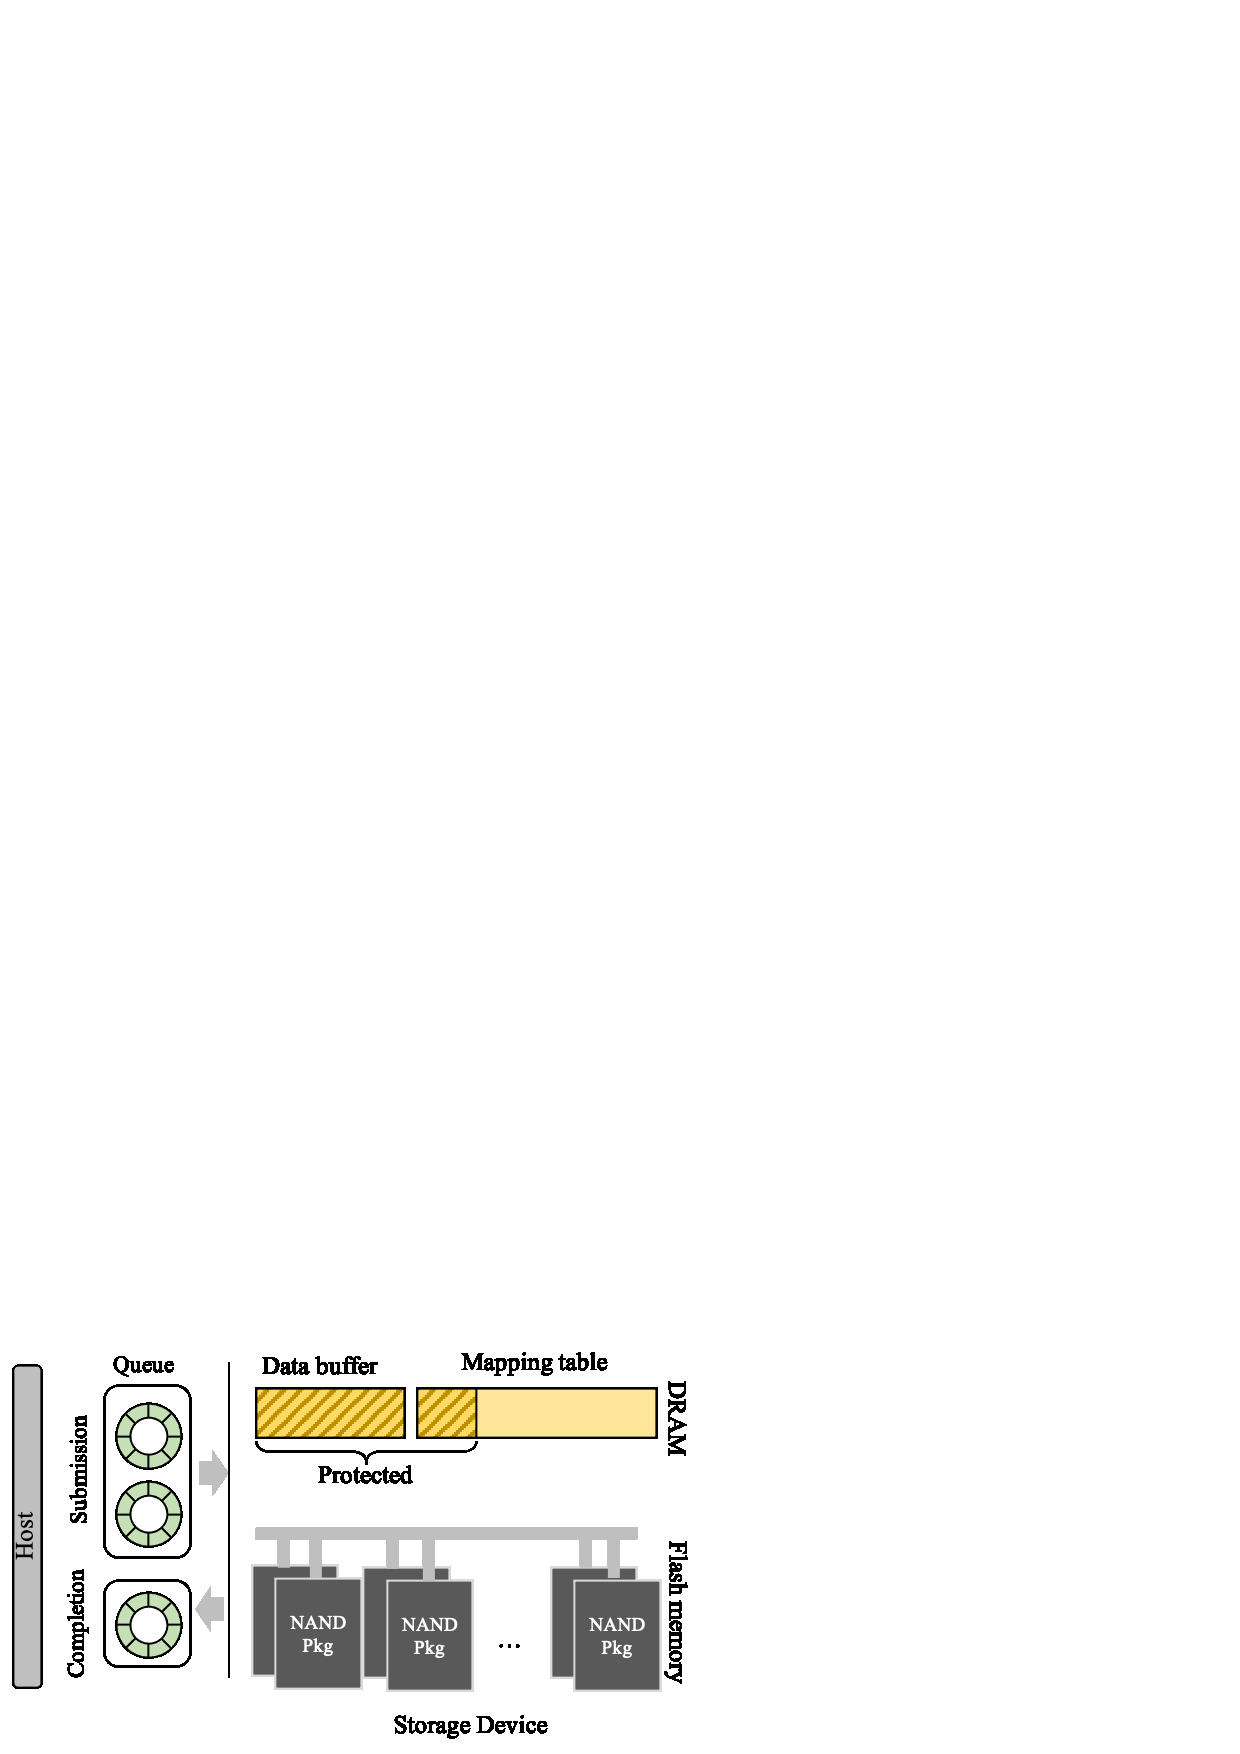
\includegraphics[width=0.4\textwidth]{figure/dawid_ssd_archi.png}
%    \caption{\textbf{Write traffic for micro benchmarks.}}
%    \centering{}
%	\subfloat[Filebench Webserver] { 
%	    \includegraphics[width=0.4\textwidth]{expr/micro/realw_1_wt.eps}
%	} 
%	\subfloat[Linkbench Run] { 
%	    \includegraphics[width=0.4\textwidth]{expr/micro/reallr_1_wt.eps}
%	}
%%    \caption{\textbf{Write traffic for macro benchmarks.}} 
%%    \label{fig_spartan_archi}
%
%    \centering{} 
%	\subfloat[TPCC] { 
%	    \includegraphics[width=0.4\textwidth]{expr/micro/realtpc_1_wt.eps}
%	} 
%    \caption{\textbf{Write traffic for macro benchmarks.}}
%    \label{fig_spartan_archi} 
%\end{figure*}

\begin{figure*}[t]
	\centering{}
		\subfloat[Random write]{ 
		    \includegraphics[width=0.4\textwidth]{expr/micro/synthr_gc.eps}
		}
	\caption{\textbf{IOPs for micro benchmarks.}} 
	
	\centering{}
		\subfloat[Linkbench_run]{
 		    \includegraphics[width=0.4\textwidth]{expr/micro/reallr_gc.eps}
		}
		\subfloat[TPCC_20]{ 
		    \includegraphics[width=0.4\textwidth]{expr/micro/realtpc_gc.eps}
		}
	
	\caption{\textbf{IOPs for macro benchmarks.}}
	\label{fig_spartan_archi} 
\end{figure*}


\begin{figure*}[t]
    \centering{}
	\subfloat[Filebench Webserver] { 
	    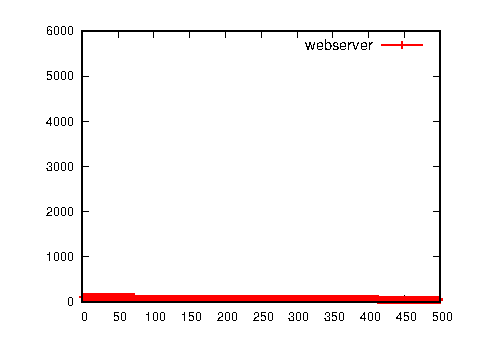
\includegraphics[width=0.4\textwidth]{webserver_uniq_500.eps}
	} 
	\subfloat[Filebench Fileserver] { 
	    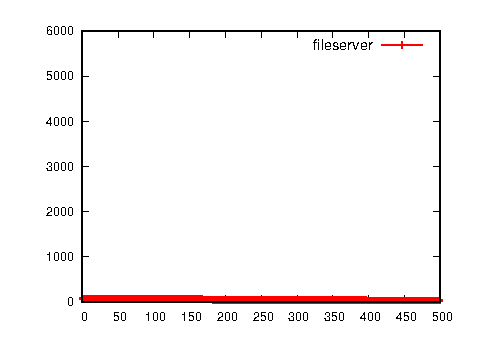
\includegraphics[width=0.4\textwidth]{fileserver_uniq_500.eps} 
	} 
    \caption{\textbf{Workload Characteristic.}}

    \centering{} 
	\subfloat[Linkbench Run] { 
	    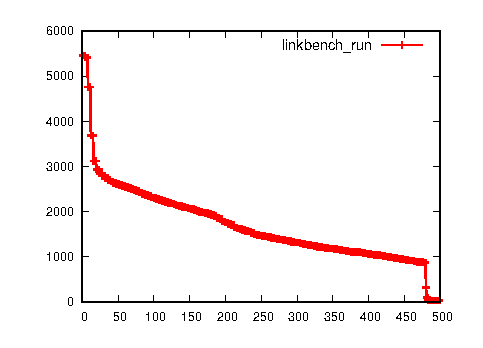
\includegraphics[width=0.4\textwidth]{linkbench_r_uniq_500.eps}
	} 
	\subfloat[TPCC] { 
	    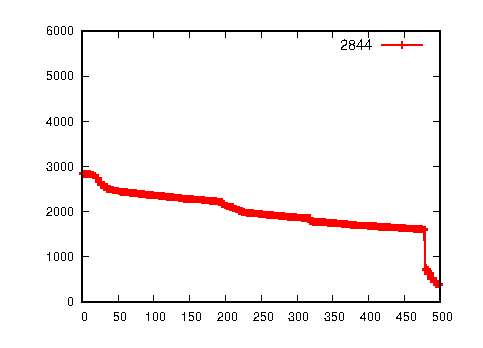
\includegraphics[width=0.4\textwidth]{tpcc_20_500.eps}
	}
    \caption{\textbf{Workload Characteristic.}}
\end{figure*} 

%\iffalse
%\begin{figure}[t]
%    \centering{}
%	\subfloat[Sequential write] {
%	    \includegraphics[width=0.4\textwidth]{expr/micro/sw_wt.eps}
%	} \\
%	\subfloat[Random write] {
%	    \includegraphics[width=0.4\textwidth]{expr/micro/rw_wt.eps}
%	}
%
%    %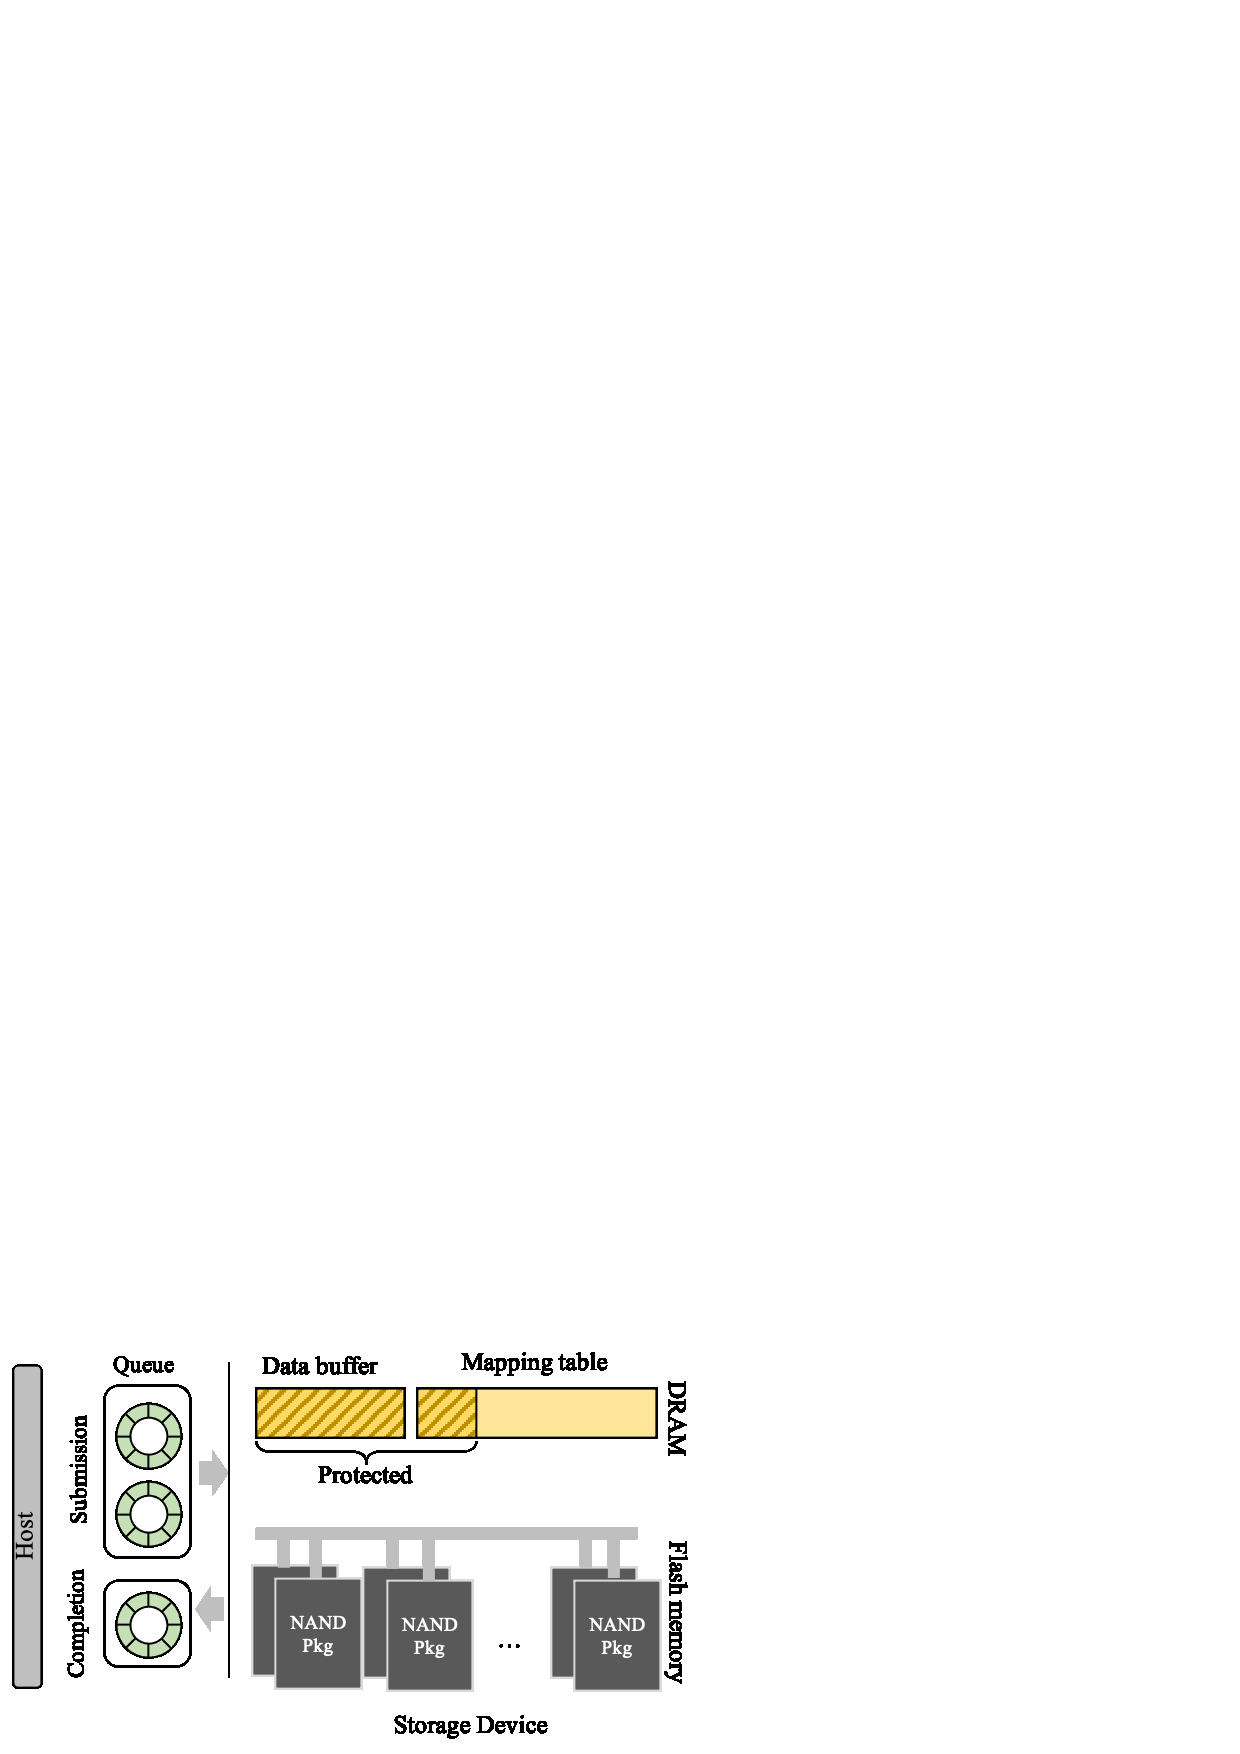
\includegraphics[width=0.4\textwidth]{figure/dawid_ssd_archi.png}
%    \caption{\textbf{Write traffic for micro benchmarks.}}
%    \label{fig_spartan_archi}
%\end{figure}
%\endif
%

\subsection{Implementation}

\subsection{Performance results}
